\documentclass[tikz,border=10pt]{standalone}
\usetikzlibrary{calc}

\begin{document}
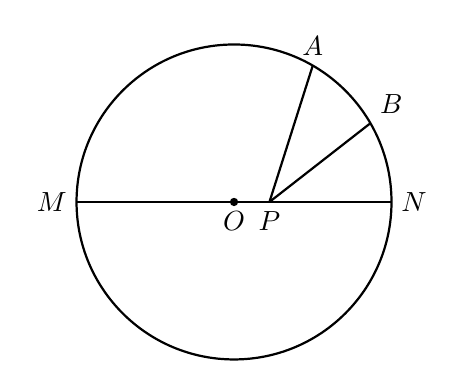
\begin{tikzpicture}
    % --- 参数定义 ---
    \def\R{2} % 定义圆的半径
    
    % --- 绘制圆 ---
    \draw[thick] (0,0) circle (\R);
    
    % --- 定义关键点坐标 ---
    \coordinate (O) at (0,0);
    \coordinate (M) at (-\R,0);
    \coordinate (N) at (\R,0);
    \coordinate (P) at (0.45,0); % P点位于半径 ON 上
    
    % 使用极坐标确定点 A 和 B 的位置 (根据视觉大致角度)
    \coordinate (A) at (60:\R);
    \coordinate (B) at (30:\R);
    
    % --- 绘制圆内的线段 ---
    \draw[thick] (M) -- (N); % 直径 MN
    \draw[thick] (P) -- (A); % 线段 PA
    \draw[thick] (P) -- (B); % 线段 PB
    
    % --- 标注点 ---
    \fill (O) circle (1.5pt); % 画出圆心 O
    \node[below] at (O) {$O$};
    \node[left] at (M) {$M$};
    \node[right] at (N) {$N$};
    \node[below] at (P) {$P$};
    \node[above] at (A) {$A$};
    \node[above right] at (B) {$B$};
    
\end{tikzpicture}
\end{document}